\begin{exercise}
      {ID-9928ff2c0f0ec6d6703eed3f2995a158a99c91dc}
      {Rohre}
  \ifproblem\problem
    \begin{minipage}{0.2\textwidth}
      \centering
      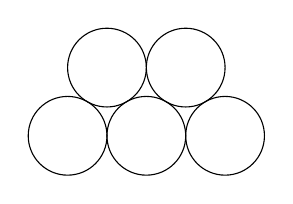
\begin{tikzpicture}
        % unten
        \draw (0, 0) circle (5mm);
        \draw (1, 0) circle (5mm);
        \draw (2, 0) circle (5mm);
        % oben
        \draw (0.5, 0.866) circle (5mm);
        \draw (1.5, 0.866) circle (5mm);
      \end{tikzpicture}%
    \end{minipage}\hfill
    \begin{minipage}{0.75\textwidth}
      Fünf Rohre mit einem Durchmesser von jeweils \simeter{1} werden auf einen Anhänger
      geladen -- drei Rohre in der unteren Reihe, zwei versetzt darüber.
      Wie hoch ist die Ladung?
    \end{minipage}
  \fi
  %\ifoutline\outline
  %\fi
  %\ifoutcome\outcome
  %\fi
\end{exercise}
